\documentclass[12pt]{article}
\usepackage[T1]{fontenc}
\usepackage[polish]{babel}
\usepackage[utf8]{inputenc}
\usepackage{lmodern}
\usepackage{float}
\selectlanguage{polish}
\usepackage{graphicx}
\usepackage{hyperref}
\usepackage{amsmath}
\title{I ty możesz zostać magistrem}
\date{\today}


\begin{document}	
\maketitle
\tableofcontents

\section{Baza Bernsteina}
Baza Bernsteina ze względu na świetne właściwości numeryczne i geometryczne jest szeroko stosowana w systemach CAD/CAM pomimo faktu, że nie jest trójkątna (traingular ???) i nie jest najszybsza w obliczeniach.\\

Ważne właściwości Bazy Bernsteina:
\begin{itemize}
	\item Formują bazę w $n+1$ wymiarowej przestrzeni $w^{n}$ wszystkich wielomianów stopnia nie większego niż $n$.
	\item Sumują się do 1 dla każdego $t \in R$
	\item Są nieujemne w przedziale $[0,1]$ i dodatnie w $(0,1)$.
	\item Sa symetryczne, tzn. $B^{n}_{i=0...n}(t) = B^{n}_{n-1}(1-t)$
\end{itemize}

\subsection{Algorytm de Casteljau}
Algorytm de Casteljau służy do obliczania wartości wielomianów w Bazie Bernsteina. Jest stabilny numerycznie. 
Niewielkim kosztem możemy uzyskąć nie tylko wartość, ale i pochodną w punkcie. Należy odczytać obie wartości algorytmu dla $n-1$ odjąć je i pomnożyć przez $n$.

\subsection{Twierdzenie Weierstrassa}
Każdą funkcję ciągłą o wartościach rzeczywistych na przedziale domkniętym $[a,b]$ można przybliżyć jednostajnie z dowolną dokładnością wielomianami Bernsteina. Im więcej punktów kontrolnych, tym większa dokładność.

\subsection{Baza Hermite'a}
Jeżeli znamy wartości na krańcach przedziału i znamy wartości pochodnych w tych punktach, to podstawiamy do wzoru i mamy aproksymację funkcji na przedziale.
\subsection{Baza Lagrange'a}
Baza nie jest triangularna (???). Można w niej interpolować.
Wielomiany Lagrange'a pozwalają nam na interpolacje punktów, bez potrzeby rozwiązywania układów współrzędnych.
\subsection{Węzły Czebyszewa}
Interpolacja w węzłach Czebyszewa jest prawie najlepsza (znika efekt Rungego).

\section{Piecewise polynomials}
\subsection{Baza B-Spline}
They are much more complex. There are two interesting properties that are not part of the Bézier basis functions, namely: (1) the domain is subdivided by knots, and (2) basis functions are not non-zero on the entire interval. In fact, each B-spline basis function is non-zero on a few adjacent subintervals and, as a result, B-spline basis functions are quite "local".

\setcounter{section}{22}
\section{Metody interpolacji obrotów}
\begin{enumerate}
	\item LERP
	\item SLERP
	\item Liniowa interpolacja kątów Eulera
	\item SQUAD - interpolacja sekwencji orientacji za pomocą wzoru
\end{enumerate}

\section{Aproksymacja obszaru obrobionego}
Obszar obrobiony możemy aproksymować za pomocą paraboloidy ściśle stycznej. 
$$d(\Delta x, \Delta y) = \frac{1}{2} [\Delta x, \Delta y] \textbf{D}  [\Delta x, \Delta y]^{T}$$
gdzie D to dwuforma (przekształcenie dwuliniowe) określająca przybliżaną powierzchnię.\\
Typowe zadanie z PUSNu: jest dana powierzchnia w postaci implicite. Sprawdź jaki maksymalny promień freza nie spowoduje podcięć lub o ile musimy się przesuwać, żeby frezować z zadaną tolerancją (żeby rowki miały maksymalnie jakąś wysokość).\\
Robimy dwuformę powierzchni i freza i je odejmujemy. Sprawdzamy czy ta dwuforma jest dodatnio określona ($X^{T}DX$ > 0, dla każdego $X$). Jeżeli tak, to nie ma podcięć. Jeżeli nie, to podcięcia mogą wystąpić, ale nie muszą (chyba trzeba sprawdzić kierunki, które chcemy frezować ???).
 
 \section{Lokalne i globalne algorytmy programowania 3C}
 Lokalne - tak jak frezowaliśmy nasze modele. APT to język do programowania urządzen sterowanych numerycznie (czyli do robienia ścieżek). Wyróżniamy w nim procedury TO/ON/PAST/TANTO (TANgential TO) oraz drive surface, part surface i check surface. PS - frezujemy stycznie do niej, DS - prowadzimy frez stycznie do niej, CS - na niej się zatrzymujemy.\\
Lokalne metody nie gwarantują ścieżek bez podcięć (collision free tool paths). Natomiast metody globalne wykluczają kolizje z ostatecznym kształtem obrabianej części. Globalne metody projektujemy poprzez wyznaczenie ITO (Inverse Tool Offset). Robimy sumę Minkowskiego przeszkód z odwórconym narzędziem w przestrzeni konfiguracji.
 
 \section{Metody rozwiązywania zadania odwrotnego prostych łańcuchów kinematycznych}
 Łańcuchy kinematyczne składają się ze zbioru sztywnych elementów połączonych za pomocą przegubów. Mamy dwa rodzaje przegubów: prismatic (przesuwające) i revolute (obracający). 
 Możemy rozwiązywać metodami explicite (jak na zajęciach): algebraiczną i geometryczną. Metodę geometryczną możemy sobie wyobrazić, co często ułatwia implementację, lecz przy bardziej skomplikowanych układach łatwiej jest w niej o błąd niż w bardziej ogólnej metodzie algebraicznej.
 Oprócz tego w przemyśle są stosowane metody numeryczne, które liczą dowolny łańcuch kinematyczny. Są wolniejsze, ale łatwiejsze do zaimplementowania.
 Do rozwiązywania zadania odwrotnego łancuchów kinematycznych stosujemy notację Denavita-Hartenberga, która upraszcza opis łańcucha.
 $$F_{i+1} = F_{i}F_{i(i+1)}$$
 $$F_{i(i+1)} = R_{x_{i}}(a_{i}) T_{x_{i}}(u_{i}) T_{z_{i+1}}(h_{i+1}) R_{z_{i+1}}(b_{i+1})$$
 
 \section{Algorytmy szukania drogi}
 Flood-Fill - jak w robocie 2D na PUSNie. Mało optymalny, łatwy w implementacji. \\
 ~\\
 PRM (Probabilistic Roadmap):
 \begin{enumerate}
 	\item Losujemy punkty w przestrzeni konfiguracji, które nie są w przeszkodach.
 	\item Próbujemy połączyć każdy punkt z każdym (czyli łączymy, gdy nie ma między nimi kolizji).
 	\item Szukamy ścieżki.
 \end{enumerate} 
Przydatną strukturą danych są kd-drzewa.\\
~\\
RRT (Rapidly-exploring random tree):
\begin{enumerate}
	\item Sprawdzamy czy wierchołek startowy jest dopuszczalny (nie jest w kolizji).
	\item Wykonujemy k kroków polegających na wylosowaniu nowej konfiguracji $q_{i}$ i łączymy ją do najbliższego wierzchołka (jeżeli nie ma kolizji).
\end{enumerate} 
 
\setcounter{section}{34}
\section{Interpolacja i aproksymacja w bazach B-spline}
\hyperlink{Prezentacja}{http://www.cad.zju.edu.cn/home/zhx/GM/009/00-bsia.pdf} 


\section{Powierzchnie obciętę i standard IGES}
Standard IGES jest standardem międzynarodowym dotyczącym danych topologicznych, geometrycznych i niegeometrzyczne (np. materiały, cechy użytkowe). Na podstawie tego standardu powstał również format pliku o tej samej nazwie pozwalający na zapisanie ponad 150 różnych typów obiektów, np. powierzchni trymowanych.

Powierzchnie obcięte składają się z dwóch części: powierzchni bazowej oraz krzywych trymowania, które wyznaczają obszary trymowania.

\section{Struktury danych reprezentacji B-rep}
%Boundary representation of models are composed of two parts: topology and geometry (surfaces, curves and points). The main topological items are: faces, edges and vertices. A face is a bounded portion of a surface; an edge is a bounded piece of a curve and a vertex lies at a point. Other elements are the shell (a set of connected faces), the loop (a circuit of edges bounding a face) and loop-edge links (also known as winged edge links or half-edges) which are used to create the edge circuits. The edges are like the edges of a table, bounding a surface portion. 
Aby uniknąć częstych obliczeń takich jak np, sprawdzenie czy punkt leży na krzywej warto zapamiętywać informacje przy tworzeniu tych struktur.


Boundary representation składa się z dwóch części: topologii oraz geometrii (powierzchnie, krzywe oraz punkty). Główne elementy topologii to: ściany (faces), krawędzie i wierzchołki. Inne elementy to powłoka (shell) - zbiór połączonych ścianek, pętla - cykl krawędzi ograniczającej ściankę, lopp-edge links (znane także jako skrzydlaczki???) - służą do tworzenia cykli z krawędzi (edge circuits). 

\begin{figure}[H]
	\centering
	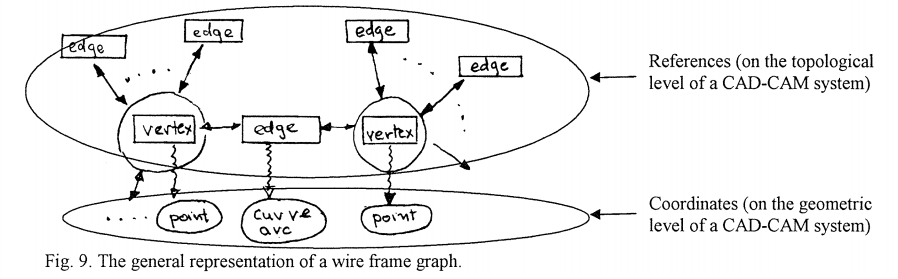
\includegraphics[scale=0.5]{Pictures/brep}
	\caption{B-rep od prof. Marciniaka}
\end{figure}

\subsection{Porównanie CSG}
CSG jest drzewem i zapamiętuje kolejne operacje wykonane na prymitywach. Jest budowane z prymitywów i podstawowych operacji boolowskich.\\
B-rep ma większą liczbę operacji, np. wyciągnięcie (extrusion) i wygładzenie krawędzi (chamfer), co pozwala na bardziej "ludzkie" tworzenie modeli.

\section{Metody lokalizacji obliczeń geometrycznych}
Przykładem problemu lokalizacji obliczeń geometrycznych jest wykrycie kolizji dwóch złożonych obiektów. Zamiast sprawdzać każdy ich element z każdym, chcemy uprościć obliczenia, odrzucając obszary, w których wiemy, że kolizja raczej nie zajdzie.

\subsection{Drzewo BSP}
Drzewo BSP (binary space partitioning) - dzielimy przestrzeń na dwie mniejsze dowolną płaszczyzną.\\
Drzewo kd - dzielimy przestrzeń na dwie mniejsze płaszczyzną ortogonalną do osi układu.\\
Octree - dzielimy przestrzeń 3D na osiem sześcianów.\\

\begin{figure}[h!]
	\centering
	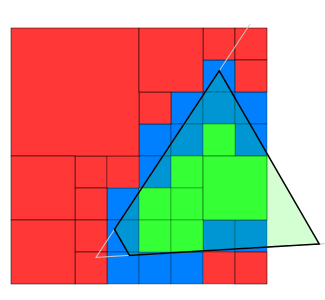
\includegraphics[scale=0.5]{Pictures/octree}
	\caption{Przykład quadtree}
\end{figure}

\section{Struktura systemu do projektowania przez podanie ograniczeń}
Zamiast sekwencyjnie rysować scenę (np. najpierw wstawiamy punkt, potem okrąg, który ma w nim środek, następnie styczną itp.), podajemy układ równań, który definiuje nam całą scenę. Jeżeli zmiennych mamy więcej niż równań to część zmiennych musi wprowadzić użytkownik jako dane wejściowe.


\section{Pojęcie naprężenia w materiale. Wektor i tensor naprężenia}
Naprężenie $\sigma$ (ang. stress) to miara gęstości powierzchniowych sił wewnętrznych, występujących w pewnym punkcie przekroju ośrodka ciągłego (ciała wolumetrycznego). Jednostką naprężenia jest paskal. Reprezentowany jako trójwymiarowy symetryczny tensor drugiego rzędu.

Wektor naprężenia $t$ to gęstość sił działających na element powierzchni w danym punkcie $P \in B$, gdzie $B$ to ośrodek ciągły (ciało). W przypadku sił wewnętrznych wartość $t$ w punkcie $P$ zależy od przekroju. Wektor $t$ jest skierowany wzdłuż wersora normalnego $n$ do powierzchni.

Po prostu: $t$ to wektor z kierunkiem $n$, a $\sigma$ to jego wartość.

\begin{equation}
t_{i} = \sigma_{ij}n_{i}
\end{equation}



\begin{figure}[H]
	\centering
	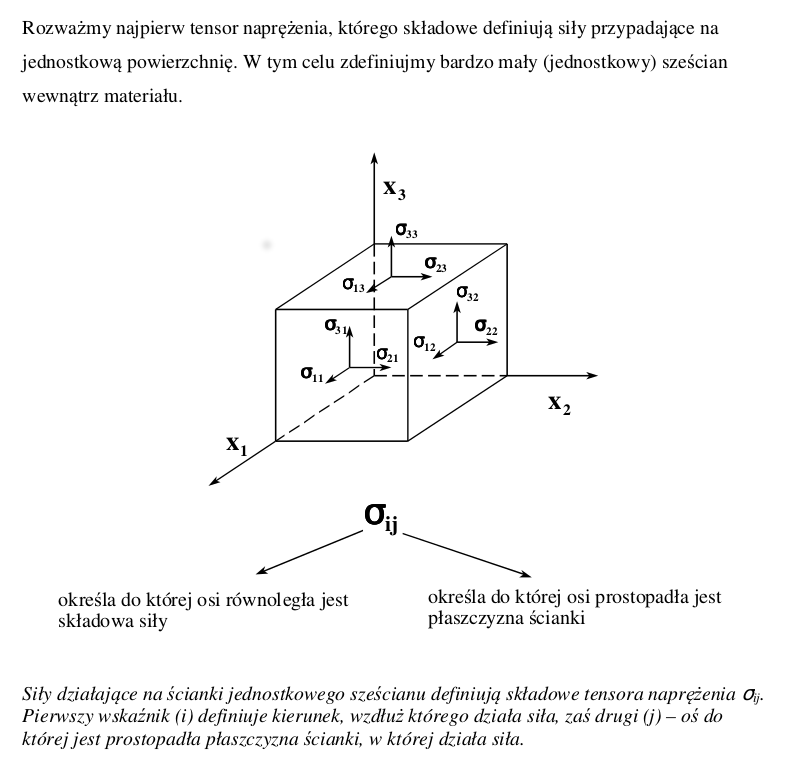
\includegraphics[scale=0.5]{Pictures/stress.png}
	\caption{}
\end{figure}

\section{Grafika Komputerowa II}


\subsection{Źródła światła}
Każde źródla światła posiada parametry: ambient, diffuse i specular

\subsubsection{Światło kierunkowe}
Światło kierunkowe (Directional light)
\begin{enumerate}
\item Reprezentowany tylko poprzez kierunek (vec3 direction)
\item Znajduje się w nieskończoności (pozycja nie ma znaczenia)
\item Wszystkie promienie światła mają taki sam kąt padania
\item Przykład: słońce
\end{enumerate}

\begin{figure}[H]
	\centering
	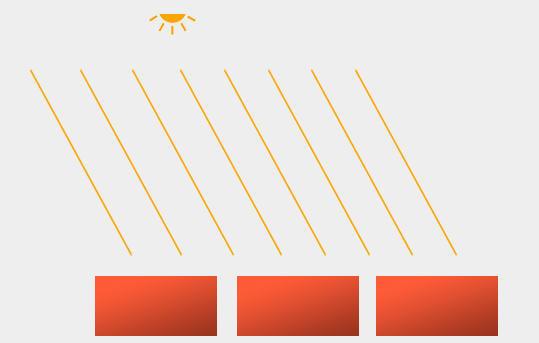
\includegraphics[scale=0.5]{Pictures/directional_light.png}
	\caption{Światło kierunkowe}
\end{figure}

\subsubsection{Światło punktowe}
Światło punktowe (Point light)
\begin{enumerate}
\item Reprezentowany tylko poprzez pozycje pozycje (vec3 position)
\item Promienie światła padają we wszystkich kierunkach
\item Tłumienie (Attenuation) światła redukuje intensywność swiatła wraz z odległościa promienia światła
\item Przykład: żarówka
\end{enumerate}

\begin{figure}[H]
	\centering
	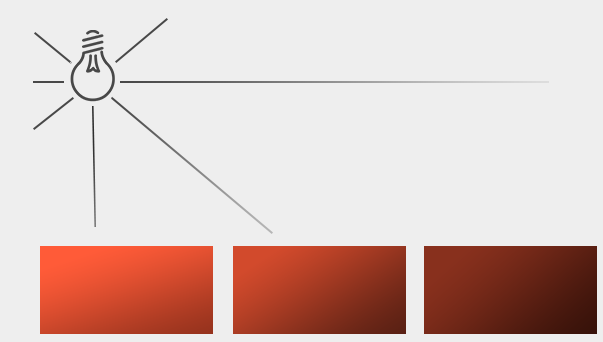
\includegraphics[scale=0.5]{Pictures/point_light.png}
	\caption{Światło punktowe}
\end{figure}

\subsubsection{Reflektor}
Reflektor (Spotlight)
\begin{enumerate}
\item Reprezentowany poprzez pozycje, kierunek i cutoff (vec3 position, vec3 direction, float cutOff)
\item Promienie padaja w danych kierunku.
\item cutOff definiuje nam promień reflektora
\item Przykład: latarka
\end{enumerate}

\begin{figure}[H]
	\centering
	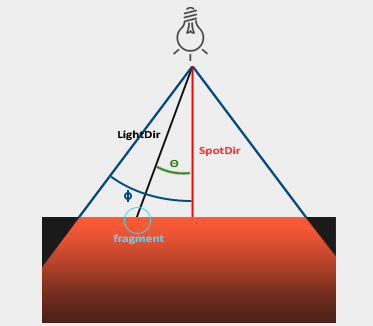
\includegraphics[scale=0.5]{Pictures/spotlight_light.png}
	\caption{Reflektor}
\end{figure}


\subsection{Oświetlenie lokalne}
Hasła związane z oświetleniem lokalnym:

\begin{enumerate}
\item Obliczanie intensywności (koloru) światła odbitego od punktu powierzchni
\item Źródła światła
\begin{enumerate}
\item kolor
\item geometria
\end{enumerate}

\item Właściwości powierzchni
\begin{enumerate}
\item kolor
\item materiał (metal, dielektryk)
\item geometra
\end{enumerate}

\item Obserwator
\end{enumerate}

Lokalne modele oświetlenia możemy podzielić na 3 typy:
\begin{enumerate}
\item Empiryczne
\item O podłożu fizycznym
\item Hybrydowe
\end{enumerate}

\subsubsection{Empiryczne}

Światło otoczenia (Ambient)
\begin{enumerate}
\item Oświetlenie tła
\item Światło oświetlające obiekt nie pochodzi z konkretnego źródła
\item Intensywność światła jednakowa we wszystkich kierunkach
\item Każdy element oświetlony w jednakowy sposób
\item Światło odbite rozchodzi się jednakowo we wszystkich kierunkach
\end{enumerate}

\begin{figure}[H]
	\centering
	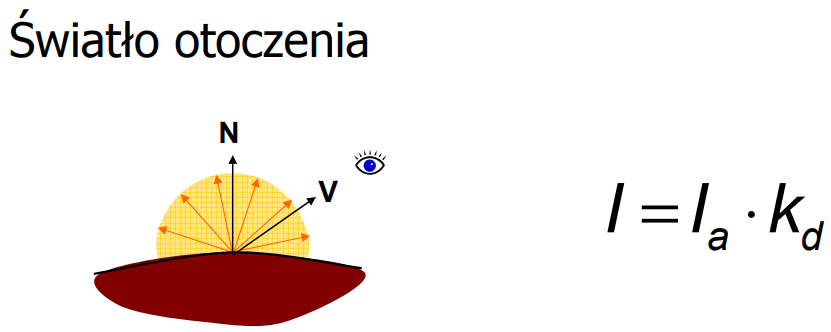
\includegraphics[scale=0.5]{Pictures/ambient.png}
	\caption{Światło otoczenia (Ambient)}
\end{figure}

Światło rozproszone (Diffuse).
\begin{enumerate}
\item Model Lamberta (odbicie lambertowskie)
\item Obiekt posiada matową powierzchnię
\item Światło odbite rozchodzi się jednakowo we wszystkich kierunkach
\item Intensywność światła odbitego zależy od kąta padania światła
\end{enumerate}

\begin{figure}[H]
	\centering
	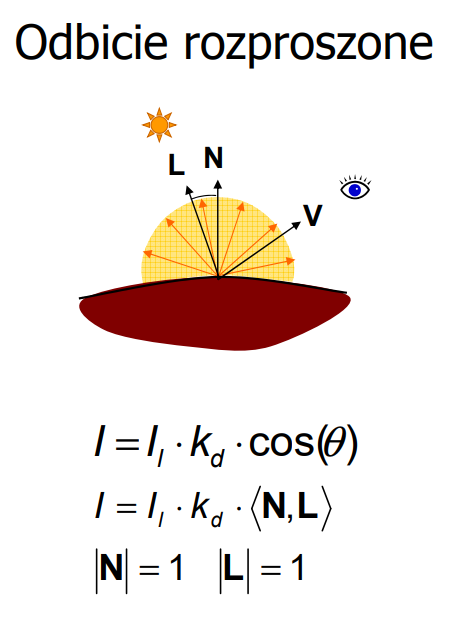
\includegraphics[scale=0.5]{Pictures/diffuse.png}
	\caption{Światło rozproszone (Diffuse)}
\end{figure}

Odbicie Zwierciadlane (Specular).
\begin{enumerate}
\item Obiekt posiada gładką powierzchnię
\item Prawo Snella: kąt odbicia jest równy kątowi padania
\item Część energii rozprasza się w innych kierunkach
\item Intensywność światła odbitego zależy od kąta padania światła i od kąta padania oka (obserwatora)
\end{enumerate}
\begin{figure}[H]
	\centering
	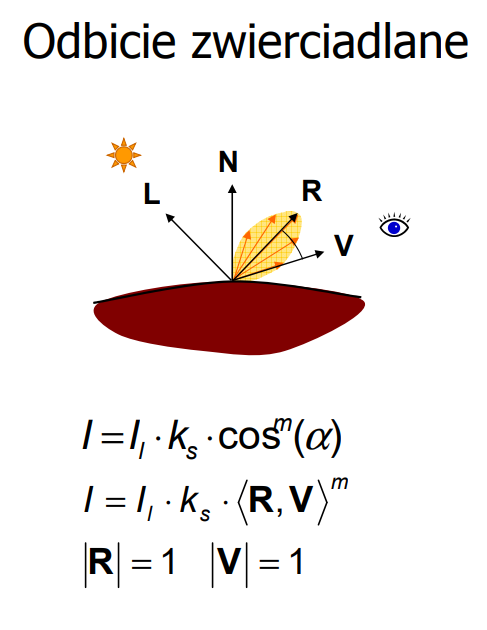
\includegraphics[scale=0.5]{Pictures/specular.png}
	\caption{Odbicie Zwierciadlane (Specular)}
\end{figure}

Model Phonga polega na połączeniu trzech komponentów: ambient, diffuse i specular.
\begin{figure}[H]
	\centering
	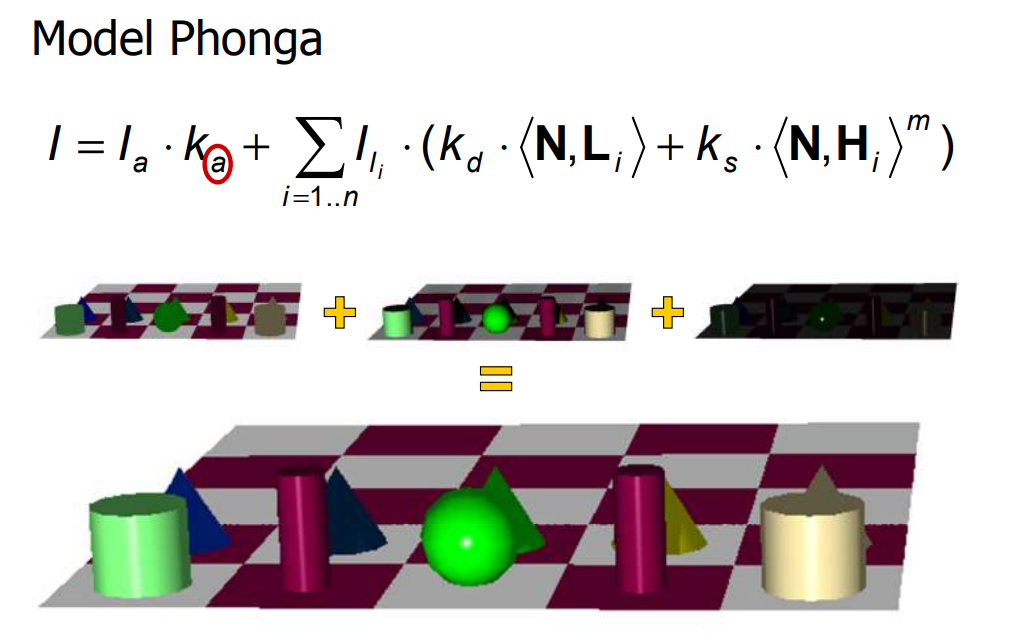
\includegraphics[scale=0.5]{Pictures/phong.png}
	\caption{Phong}
\end{figure}

\subsubsection{O podłożu fizycznym}

\subsubsection{Hybrydowe}

\subsection{Oświetlenie globalne}

\subsection{Porównanie}
\begin{figure}[H]
	\centering
	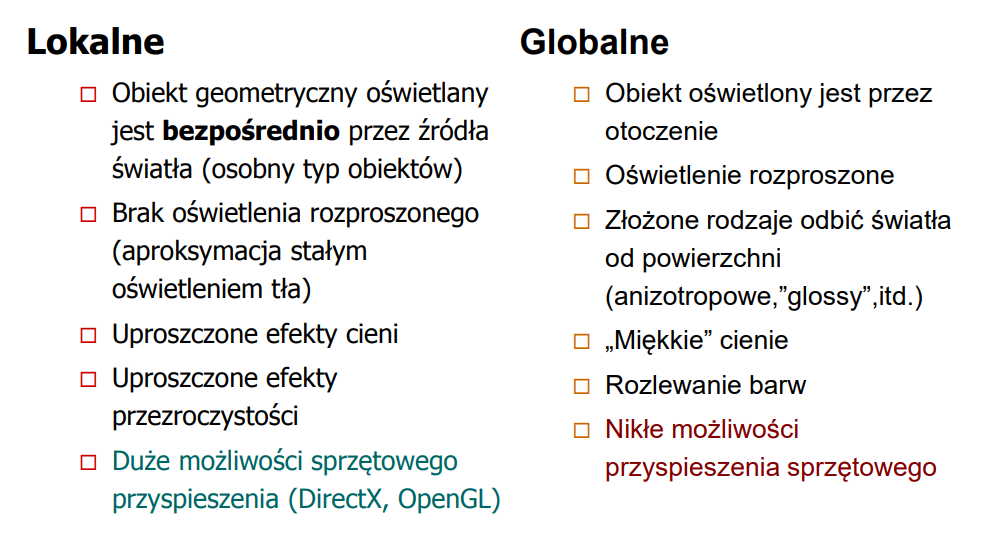
\includegraphics[scale=0.5]{Pictures/oswietlenie.png}
	\caption{}
\end{figure}


\section{Algebra Zewnętrzna}

\subsection{Forma różniczkowa (k-forma)}
Forma różniczkowa albo k-forma to tensor rzędu $k$, który jest antysymetryczny względem wymiany par indeksów. 1-form $\omega_{1}$ o wymiarze $n$:
\begin{equation}
\omega_{1} = a_{1} dx_{1} + a_{2} dx_{2} + ... + a_{n} dx_{n} = a_{i} dx_{i}
\end{equation}
gdzie $a_{i}$ są funkcjami $a_{i}(x_{1}, x_{2}, ..., x_{n})$

Przykład 2-formy:
\begin{equation}
\omega_{2} = a_{1} dx_{1} \wedge dx_{2} + a_{2} dx_{1} \wedge dx_{3} + a_{3} dx_{2} \wedge dx_{3}
\end{equation}
gdzie operator $(\cdot) \wedge (\cdot)$ to iloczyn zewnętrzny zdefiniowany:
\begin{enumerate}
\item $t \wedge s = - s \wedge t$
\item $t \wedge t = 0$
\item $t \wedge (r + s) = t \wedge r + t \wedge s$
\end{enumerate}

\subsection{Pochodna zewnętrzna}
Pochodna zewnętrzna k-formy $\omega$ to $k+1$-forma $d \omega$.
Jeśli 1-forma $\omega$ to:

\begin{equation}
\omega = a dx + b dy
\end{equation}

wtedy $d \omega$ jest zdefiniowane jako:
\begin{align*}
d \omega = d(a dx + b dy) = [\frac{\partial a}{\partial x} (dx \wedge dx) + \frac{\partial a}{\partial y} (dy \wedge dx)] + [\frac{\partial b}{\partial x} (dx \wedge dy) + \frac{\partial b}{\partial y} (dy \wedge dy)] =
\\
\frac{\partial a}{\partial y} (dy \wedge dx) + \frac{\partial b}{\partial x} (dx \wedge dy)
\end{align*}

\subsection{Dywergencja}
Dywergencja pola wektorowego to operator różniczkowy przyporządkowujący trójwymiarowemu (dwuwymiarowy też) polu wektorowemu pole skalarne będące formalnym iloczynem skalarnym operatora nabla $\nabla$ z polem. 

Dywergencja to miara ilości strumienia wchodzącego lub wychodzącego z punktu. Dywergencja to tempo ekspansji (ang. expansion, positive divergence) lub skurczania (ang. contraction, negative divergence) się strumienia.

Jeśli dany punkt zobaczy strumień, który do niego wchodzi to zacznie krzyczeć, że wszystko się zbliża (ang. negative divergence). Jeśli dany punkt zobaczy strumień, który z niego wychodzi to zacznie krzyczeć, że wszystko sie od niego oddala (ang. positive divergence).

\begin{figure}[H]
	\centering
	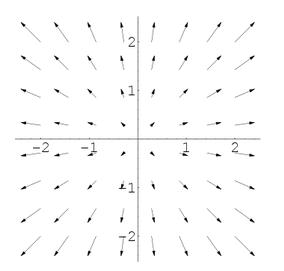
\includegraphics[scale=1.0]{Pictures/vector_field_div.png}
	\caption{Przykład pola wektorowego pokazujący prędkość strumienia cieczy. Strumień oddala się od początku ukladu współrzędnych (ekspansja). Ta ekspansja (ang. expansion) jest udowodniona przez dodatnią wartość dywergencji div F}
\end{figure}

\subsection{Twierdzenie Stokesa}
Całka formy różniczkowej (k-formy) $\omega$ na brzegu $\partial \Omega$ jakieś rozmaitości (manifold) jest równa całce pochodnej zewnętrznej $d \omega$ na całości $\Omega$

\begin{equation}
\int_{\partial \Omega} \omega = \int_{\Omega} d \omega
\end{equation}

Twierdzenie Gaussa-Ostrogradskiego, podstawowe twierdzenie rachunku całkowego (Fundamental theorem of calculus) i twierdzenie Greena są specjalnymi przypadkami twierdzenia Stokesa.

Tw. Stokesa umożliwia nam zamianę całki powierzchniowej na objętościową (i na odwrót)

\subsection{Twierdzenie Gaussa-Ostrogradskiego}

Znane także jako twierdzenie o dywergencji (Divergence theorem).
Specjalny przypadek tw. Stokesa, w którym funkcja podcałkowa po objętości to dywergencja pola wektorowego $F$

\begin{equation}
\int_{V} (\nabla \cdot F) dV = \int_{\partial V} (F \cdot n) dA
\end{equation}

$F$ to pole wektorowe zdefiniowane w sąsiedztwie $V$. $n$ to pole normalnych (skierowanych na zewnątrz, ang. outward) do brzegu $\partial V$.

Załóżmy, że chcemy napompować koło samochodowe, które jest idealną bryła sztywną (koło nie rozszerzy się po dodaniu powietrza). Co się stanie z powietrzem w środku koła? Powietrzne w środku koła skurczy się.

Jeśli $F$ to pole wektorowe reprezentujące strumień cieczy to dywergencja div $F$ reprezentuje ekspansję lub skurczanie sie tej cieczy. Tw. o dywergencji mówi, że całkowita ekspansja strumienia cieczy w jakims trójwymiarowym regionie $V$ jest równa całkowitemu strumieniowi cieczy na zewnątrz brzegu $V$.

W naszym przykładzie koło stanowi region $V$. Pompowanie powietrza do środka koła w kierunki przeciwnym do normalnej $n$ daje nam ujemna wartość $\int_{\partial V} (F \cdot n) dA$. Co oznacza, że wartość $\int_{V} (\nabla \cdot F) dV$ też jest ujemna, co oznacza, że powietrze skurczyło się. Dokładnie to co założyliśmy.

\section{Projektowanie środowiska wirtuanego}

\subsection{Porównanie mechanik}
Wszystkie mechaniki są sobie równoważne. Różnią się łatwością zapisu równań dla różnych przypadków.\\
~\\
\textbf{Mechanika Newtona} $F = ma$. Jest dobra do systemów cząsteczkowych. Równania zależą od układu współrzędnych, w szczególności czy jest inercyjny (Wojtek patrzy na karuzelę) czy nieinercyjny (Wojtek siedzi na karuzeli). Ciężko w nim uwzględnić ograniczenia. W przypadku bryły sztywnej oprócz ruchu postępowego mamy też ruch obrotowy, który jest wyrażony wzorem $M = I\omega$. \\
~\\
\textbf{Mechanika d'Alamberta} ułatwia wprowadzenie ograniczeń, ale przez to wzrasta nam liczba zmiennych i równań w układzie. Gdy mamy $M$ parametrów i $U$ ograniczeń, to mamy $M + U$ równań.
W tej mechanice mamy równania DAE (różniczkowo-algebraiczne): $U$ algebraicznych i $M$ różniczkowych.
\begin{equation} 	
	\begin{bmatrix}
	m_{1}  &   &   &  
	\\[0.3em]
	  & m_{1} &  &   
	\\[0.3em]
	  &  & m_{2} &  
	  \\[0.3em]
	  &  &  & m_{2}
	\end{bmatrix}
	\begin{bmatrix}
	\ddot{x_{1}}  
	\\[0.3em]
	\ddot{y_{1}}   
	\\[0.3em]
	\ddot{x_{2}}  
	\\[0.3em]
	\ddot{y_{2}}
	\end{bmatrix}
	= F + \lambda _{i} G_{i}	
\end{equation}
gdzie: \\
$i=1:U$ \\
$G_{i}$ - gradient i-tego ograniczenia \\
~\\
\textbf{Zasada prac wirtualnych} redukuje liczbę równań w mechanice d'Alamberta. Aby ją zastosować, należy wziąć wektor $v$ z przestrzeni stycznej do wszystkich ograniczeń. Siły reakcji w d'Alambercie są prostopadłe do ograniczeń, więc taki magiczny wektor $v$ nam je wszystkie wyzeruje. Dzięki temu upraszczamy układ, a liczba równań spada do $M - U$.\\
~\\
\textbf{Mechanika Lagrange'a} jest niezależna od układu współrzędnych. Dzięki temu możemy łatwo rozwiązywać skomplikowane układy ruchu - musimy tylko opisać parametryzację. Mechanika Lagrange'a bazuje na energii układu. 
$$ \dfrac{d}{dt} (\dfrac{\partial L}{\partial\dot{Q_{i}}}) - \dfrac{\partial L}{\partial Q_{i}} = 0$$
gdzie: \\
$L = T - U$ -- funkcja Lagrange'a\\
$T$ -- energia kinetyczna \\
$U$ -- energia potencjalna \\
$Q_{i}$ -- współrzędne parametryzacji\\
~\\
\textbf{Mechanika Hamiltona} podobnie jak w mechanice Lagrange'a potrzebujemy energii i parametryzacji. Jednak zamiast jednego równania drugiego rzedu mamy dwa równania pierwszego. Mechanika Hamiltona jest połączeniem mechaniki klasycznej z mechaniką kwantową.
$$ \dot{p_{i}} = - \dfrac{\partial H}{\partial q_{i}} + D $$
$$ \dot{q_{i}} = - \dfrac{\partial H}{\partial p_{i}} $$
gdzie: \\
$H = T + U $ -- funkcja Hamiltona
$T$ -- energia kinetyczna \\
$U$ -- energia potencjalna \\
$p_{i}$ -- współrzędne pędu
$q_{i}$ -- współrzędne parametryzacji

\subsection{Systemy dynamiczne}
\textbf{System dynamiczny} gładkie pole wektorowe na N-wymiarowej rozmaitości różniczkowej zwanej przestrzenią stanów systemu. Każdy stan należący do tej przestrzenii może zmieniać się w czasie zgodnie z funkcją zmiany stanu (równaniem różniczkowym). \\
System dynamiczny nie zależy od czasu, to wtedy jest autonomiczny. \\
Jeżeli funkcja zmiany stanu jest liniowa i system jest autonomiczny to jest to system LTI (Linear Time Invariant).\\
~\\
\subsubsection{Stabilność}
Na przykładzie wahadła: mamy dwa punkty równowagi - na górze i na dole. Górny nie jest stabilny, bo po wytrąceniu wahadła z tego położenia nigdy do niego nie wrócimy. Punkt na dole jest stabilny, bo wahadło do niego wraca. Stabilność z definicji oznacza, że po wytrąceniu wahadło wróci w otoczenie punktu równowagi. Jednak nasz punkt na dole wahadła jest "bardziej" stabilny, ponieważ jest stabilny asymptotycznie. Znaczy to, że wraz z upływem czasu zawsze zbliża się on do punktu równowagi (granica dązy do 0). W praktyce wiemy, że takie wahadło wróci dokładnie do punktu równowagi, a nie zatrzyma się gdzieś obok. Do sprawdzania czy punkt jest stabilny może nam posłużyć kryterium Lyapunova.\\

 \subsection{Sterowanie}
 System sterowania jest to system dynamiczny z dodatkowym zbiorem parametrów $u$, za pomocą których możemy zmieniać pole wektorowe (trajektorię) systemu. \\
 ~\\
 \textbf{Bang-Bang} - głupie sterowanie, włączamy i wyłączamy na zmianę.\\
 ~\\
 \textbf{Open loop control} - system kontroli, w którym $u$ jest obliczane tylko na podstawie modelu systemu. Oznacza to, że kontroler nie obserwuje wyjścia, co w praktyce prowadzi do tego, że system nie poprawia błędów na wyjściu. Nie poprawia też zaburzeń. Jest przydatny gdy dokładnie znamy pole wektorowe i pożądaną trajektorię. Przykładowo się go stosuje w silniku krokowym sterującym ramieniem robota.\\
 ~\\
 \textbf{Closed loop control} - jest to open loop control z dodanym regulatorem, czyli do wyznaczenia $u$ bierzemy także wyjście z poprzedniej iteracji i wyjście idealne, do którego dążymy (wcześniej zadane). W ten sposób staramy się kompensować błędy na wyjściu. Przykład: autopilot w samolocie. Mamy zadaną trajektorię, po której chcemy lecieć. Co krok porównujemy wyjście z tą trajektorią i jeżeli są odstępstwa to poprawiamy.\\
 ~\\
 Open loop control służy do minimalizacji jakiegoś kryterium (np. odległości trafienia rakiety od samolotu) i do przejścia ze stanu początkowego w dany stan końcowy. Closed loop control pilnuje nam, żeby system nie przestał być stabilny (dzięki poprawianiu błędów).\\
 ~\\
 \textbf{Stany równowagi} - przekształcamy układ tak, żeby mieć tylko równania pierwszego rzędu (możemy wstawiać nowe zmienne, np. $v = \dot{x}$). I dla wszystkich $\dot{x} = 0$ mamy stany równowagi.\\
 ~\\
 \textbf{Bifurkacja} - zmiana właściwości układu dla pewnych wartości. Przykład dla paraboli: ma dwa miejsca zerowe. Jednak jeśli współczynnik przy $x^{2}$ wynosi 0, to funkcja jest liniowa i ma tylko jeden pierwiatek.\\
 
 \subsection{Linearyzacja}
 Linearyzacja umożliwia nam analizę systemu nieliniowego w otoczeniu jakiegoś punktu. Linearyzacja funkcji pierwszego rzędu to szereg Taylora wokół punktu. Gdy linearyzujemy wokół punktu równowagi, macierze są stałe. W innych punktach mogą one zależeć od parametrów.

\subsection{Transformata Laplace'a}
Transformata Laplace'a pozwala nam przejść z równań różniczkowych określonyw w dziedzinie rzeczywistej, do równań algebraicznych w zespolonych. W ten sposób możemy obliczyć pierwiastki, a następnie za pomocą odwróconej tranformaty wracamy do dziedziny rzeczywistej. Odwrotna transformata jest słaba numerycznie, więc oblicza się ją symbolicznie lub sprawdza wartości w tabelach. Transformatę Laplace'a stosujemy tylko do liniowych równań różniczkowych ze stałymi współczynnikami (czyli LTI w rozumieniu z ćwiczeń). 

\subsection{Stabilność układu LTI}
Możemy pierwiastki wielomianu charakterystycznego. Jeżeli ich części rzeczywiste są mniejsze od zera to układ jest asymptotycznie stabilny. Możemy także to sprawdzić za pomocą Kryterium Routha lub Kryterium Hurvitza. Kryterium Routha - liczymy wielomian charakterystyczny. Jeżeli wszystkie współczynniki wielomianu są większe od zera i wszystkie elementy z pierwszej kolumny macierzy trójkątnej Routha też są większe od zera to system jest asymptotycznie stabilny. Kryterium Hurvitza: bierzemy wielomian charakterystyczny i jego współczynniki wkładamy do macierzy. Układ jest stabilny, gdy $a_{n} > 0$ i główne minory macierzy są dodatnie.

\subsection{Kontrolowalność}
System musi być kontrolowalny, żebyśmy mogli zrobić z systemem co chcemy za pomocą wejścia.\\
System jest kontrolowalny, gdy dowolny stan końcowy jest osiągalny z dowolnego stanu początkowego w skończonym czasie. Kontrolowalność systemu LTI sprawdzamy za pomocą własności: $$Rank[A|B] = n$$ gdzie $$[A|B] = [B, AB, A^{2}B,...,A^{n-1}B]$$

\subsection{Obserwowalność}
System jest obserwowalny, gdy stan początkowy $x(0)$ może być jednoznacznie wyznaczony na podstawie wiedzy o wejściu $u(t)$ i wyjściu $y(t)$ dla wszystkich $t$ pomiędzy 0 i dowolnym skończonym $T$. Obserwowalność systemu LTI sprawdzamy za pomocą własności: $$Rank[A^{T} | C^{T}] = n$$ gdzie $$[A^{T} | C^{T}] = [C^{T}, A^{T}C^{T},(A^{T})^{2}C^{T},...,(A^{T})^{n-1}C^{T}]$$
~\\
Jeżeli system jest kontrolowalny i obserwowalny to \textbf{istnieje kontroler}, który stabilizuje system wzdłuż pożądanej trajektorii.

\subsection{Serwomechanizm}
Serwomechanizm jest jak closed loop control tylko, że nie tylko stabilizuje system i kompensuje odchylenia, ale także liczy pożądaną kontrolę. Jest szeroko wykorzystywany w praktyce, np. w sterowaniu łodzią.

\subsection{PID}
Kontroler PID (proportional-integral-derivative) - kontroler zawierający trzy człony poprawiające. 
\begin{enumerate}
	\item Proporcjonalny jest po to, żeby dawać wejście proporcjonalne do błędu (w Bang-Bang zawsze dawaliśmy max lub min, co było bezsensu; P nam to poprawia). Czyli kompensuje błąd bieżący.
	\item Itegral (całkowy) Kompensuje akumulację błędów z przeszłości.
	\item Derivative (różniczkowy) kompensuje przewidywanie błędy w przyszłości.
\end{enumerate}
PID jest najczęściej stosowanym kontrolerem.

\subsection{LQR}
Linear-Quadratic regulator jest regulatorem optymalnym, czyli lepszym niż PID. Może być stosowany, gdy system dynamiczny jest opisany liniowym równaniem różniczkowym i koszt (który minimalizujemy) jest dany funkcją kwadratową.

\section{Programowanie matematyczne}
\subsection{Programowanie liniowe z ograniczeniami}
Rozwiązań ZPL należy szukać w wartościach ekstremalnych (wierzchołkach) zbioru ograniczeń.\\

\textbf{Sympleks}:
\begin{enumerate}
	\item Wybieramy BRD (bazowe rozwiązanie dopuszczalne): dopełniamy ograniczenia do postaci standardowej, żeby były równości. Zmienne dopełniające tworzą BRD. Jeżeli rozwiązanie mamy dane z równościami to możemy albo wybrać macierz jednostkową albo musimy dodać zmienne sztuczne. Jeżeli dodaliśmy zmienne sztuczne to musimy rozwiązać zadanie metodą dwufazową lub metodą kar ("dużego M"). W metodzie "dużego M" robimy sympleks raz, ale mamy inne drzewo interpretacji.
	\item \label{petla} Obliczamy wskaźniki optymalności ($z_{j} - c_{j}$).
	\item Jeżeli $z_{j} - c_{j} \geq 0 \forall j = 1,2,...,n$ to aktualne BRD jest optymalne --- STOP.
	\item Badamy współczynniki $a_{ij}$. Jeżeli $ \exists j z_{j} - c_{j} < 0$, przy którym $a_{ij} \leq 0$ dla $i \in B$, to zadanie nie posiada skończonego rozwiązania optymalniego --- STOP
	\item Szukamy niebazowej zmiennej, która wejdzie do bazy nowego BRD za pomocą kryterium wejścia  $z_{k} - c_{k} = min\{ z_{j} - c_{j}\}$.
	\item Stosując kryterium wyjścia $\frac{b_{r}}{a_{rk}} = min{\frac{b_{i}}{a_{ik}}}$, znaleźć indeks zmiennej usuwanej z aktualnego BRD.
	\item Uaktualniamy tabelkę (liczymy nowe BRD dla sąsiedniej bazy i obliczamy nowe $a_{ij}$).
	\item Wracamy do \ref{petla}.
\end{enumerate}

~\\
\textbf{Reguła Blanda} chroni przed zapętlaniem się sympleksu (może się zapętlić gdy mamy zdegenerowane BRD -- co najmniej jedna ze składowych części bazowej jest równa zeru). Od zwykłego sympleksu różni się innym kryterium wejścia i wyjścia (po prostu bierzemy najmniejszy indeks).\\
~\\
Zalety i wady sympleksu:
\begin{enumerate}
	\item Ogólnie znany i często stosowany do rozwiązywania ZPL w praktyce.
	\item Złożoność pesymistyczna: wykładnicza (metoda punktu wewnętrznego wielomianowa).
	\item Złożoność średnia: liniowa O((m+n)/2).
\end{enumerate}
~\\
\textbf{Zadanie dualne}: jeśli ZPL posiada dużą liczbę ograniczeń, a niewielką liczbę zmiennych ($m>n$), to warto zamiast niego rozważać zadanie dualne o niewielkiej liczbie ograniczeń i zwiększonej liczbie zmiennych decyzyjnych. Aby przejść do zadania dualnego zamieniamy: max na min, zmienne na ograniczenia i ograniczenia na zmienne.\\
~\\
\textbf{Warunek komplementarności}
Niech $\bar{x} = (x, x^{d})$ oraz $\bar{y} = (y, y^{d})$ -- BRD odpowiednio dla ZP i ZD. Rozwiązania te są optymalne, gdy $x^{T}y^{d} + y^{T}x^{d} = 0$. Za pomocą warunku komplementarności możemy sprawdzić czy rozwiązanie jest optymalne (układ równań i rozkminy).
\begin{figure}[H]
	\centering
	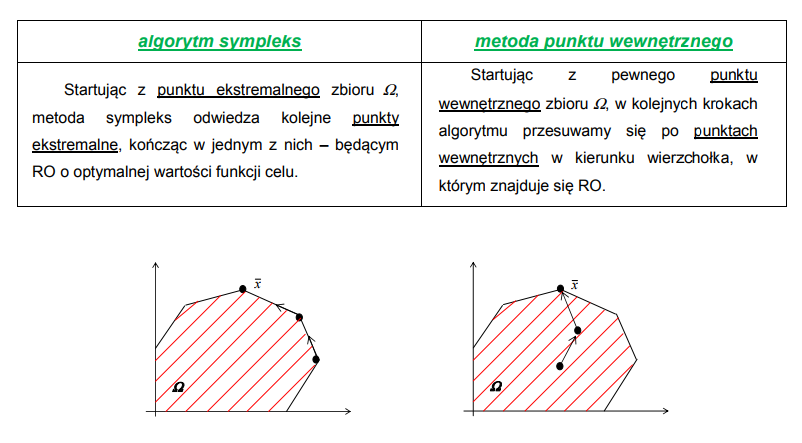
\includegraphics[scale=0.7]{Pictures/sympleks_metodaPunWew}
	\caption{Porównanie algorytmu sympleksu z metodą punktu wewnętrznego}
\end{figure}

\textbf{Mnożniki Lagrange'a}\\
Za pomocą Mnożników Lagrange'a sprawdzamy czy dane rozwiązanie jest RO (rozwiązaniem optymalnym). Funkcja musi być wypukła. Dla danego rozwiązania $x$ i dla zadanych ograniczeń sprawdzamy, czy są one aktywne. Są aktywne, gdy po wstawieniu do nich $x$ zachodzi równość. Korzystając ze wzoru obliczamy $\lambda$ i jeżeli dla każdego ograniczenia aktywnego $ \lambda \geq 0$ to $x$ jest RO.

\subsection{Optymalizacja nieliniowa bez ograniczeń}
Ekstremum funkcji mamy, gdy gradient jest równy 0. Jeżeli funkcja jest $C^{2}$ to możemy obliczyć jej Hessian (macierz drugich pochodnych) i sprawdzić jego określoność. W ten sposób sprawdzamy czy ekstremum jest minimum czy maksimum. 

\begin{figure}[H]
	\centering
	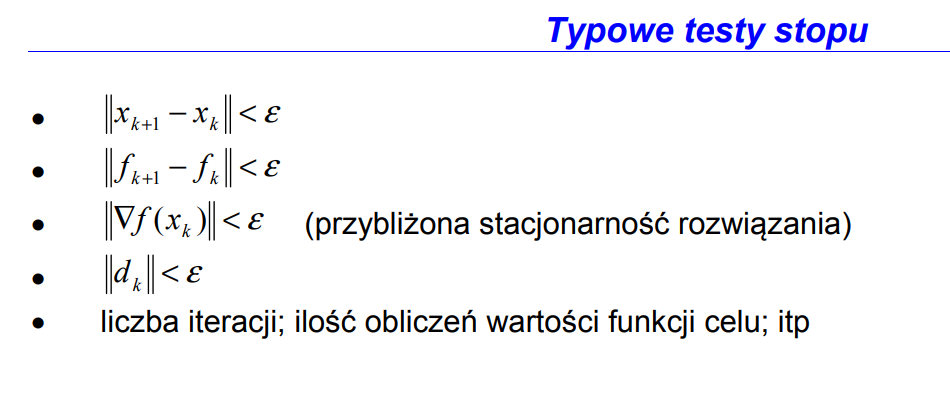
\includegraphics[scale=0.7]{Pictures/warunki_stopu}
	\caption{Typowe warunki stopu}
\end{figure}

\textbf{Algorytmy optymalizacji nieliniowej bez ograniczeń}\\
Każdy algorytm składa się z dwóch etapów. W pierwszym znajdujemy kierunek poszukiwań $d_{k}$, a w drugim długość kierunku $\alpha _{k}$.\\

Metody minimalizacji jednokierunkowej (szukania $\alpha$):
\begin{enumerate}
	\item Analityczna -- obliczenia symboliczne, dobre dla funkcji "prostej" postaci.
	\item Eliminacji przedziałów (funkcja musi być unimodalna):
	\begin{enumerate}
		\item Metoda dychotomii (dwudzielności) -- jak wyszukiwanie binarne tylko lekko zmodyfikowane. W każdej iteracji obliczamy dwie wartości funkcji i usuwamy połowę przedziału.
		\item Metoda złotego podziału -- wybieramy dwa punkty próbne w przedziale. W każdej iteracji obliczamy tylko jedną wartość funkcji i zmniejszamy przedział o współczynnik $c$.
		\item Metoda Fibonacciego
		\item Metoda punktu środkowego
	\end{enumerate}
	\item Interpolacja funkcji celu:
	\begin{enumerate}
		\item Metoda Newtona
		\item Interpolacja paraboliczna
	\end{enumerate}
	\item Metody przybliżone:
	\begin{enumerate}
		\item Testy Goldsteina
		\item Algorytm Armijo
	\end{enumerate}
\end{enumerate}

\textbf{Metody optymalizacji nieliniowej bez ograniczeń}:
\begin{enumerate}
	\item Bezgradientowa: Gaussa-Seidela: $d_{i} = e_{i}$. W każdej iteracji idziemy w $n$ kierunkach bazowych i sprawdzamy czy jesteśmy w optimum. Uwagi: prosta obliczeniowo, wolno zbieżna, może zygzakować. Jest to gorsza wersja gradientów sprzężonych.
	\item Gradientowe:
	\begin{enumerate}
		\item Metoda gradientu prostego: $d_{k} = -\nabla f(x_{k})$, $\alpha _{k} = const$.
		\item Metoda najszybszego spadku: $d_{k} = -\nabla f(x_{k})$, $\alpha _{k}$ -- na podstawie dokładnej lub przybliżonej minimalizacji kierunkowej. Uwagi: zbieżność liniowa, relatywnie najszybsze zbliżanie się do RO (podczas początkowych kroków), wolna zbieżność (zygzakowanie, czyli każdy kolejny kierunek jest do siebie prostopadły -- wynika to z tego, że $\alpha$ jest minimalna), wrażliwa na błędy zaokrągleń.
		\item \label{gradientsprzezony} Metoda gradientu sprzężonego: aby nie wybierać tego samego kierunku dwa razy (czyli usunąć zygzakowanie), szukamy zbioru kierunków A-sprzężonych, czyli zmieniamy układ współrzędnych. Dzięki temu dojdziemy do rozwiązania w maksymalnie $n$ krokach (każdy z kierunków jest wykorzystywany tylko raz) dla funkcji kwadratowej. Dzięki tej metodzie możemy też rozwiązać układ równań liniowych $Ax = b$, gdzie $A$ jest symetryczna i dodatnio określona.
	\end{enumerate}
	\item Gradientowe drugiego rzędu:
	\begin{enumerate}
		\item Metoda Newtona: funkcja $C^{2}$. Przybliżamy funkcję $F$ parabolą w punkcie (gdzie $F(\delta) = f(x_{x} + \delta)$, $\delta$ - krok i liczymy jej ekstremum. Jest zbieżny kwadratowo (czyli szybki), ale większy nakład obliczeniowy w każdym kroku. W każdej iteracji obliczenie kierunku uwzględnia odwrócenie Hesjana.
		\begin{figure}[H]
			\centering
			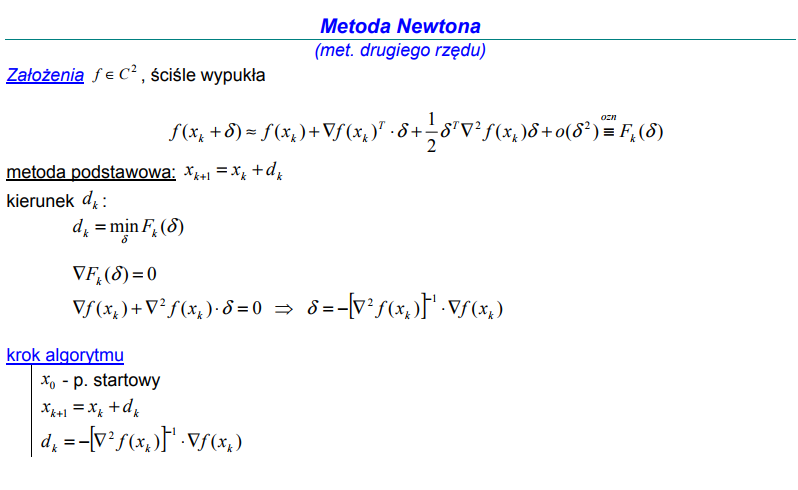
\includegraphics[scale=0.7]{Pictures/metoda_newtona}
			\caption{Metoda Newtona}
		\end{figure}
		\item Metoda Newtona-Raphsona -- jak Metoda Newtona, tylko minimalizujemy jeszcze $\alpha$. Dzięki temu mamy większe obszary zbieżności.
		\item Metoda quasi-Newtonowskie -- liczymy odwrotność Hesjana tylko raz, potem co pętle go poprawiamy. Metody poprawiania: DFP, BGFS. 
	\end{enumerate}
\end{enumerate}
~\\
\textbf{Metoda pełzającego sympleksu} to metoda bezpośrednia heurystyczna.
\begin{figure}[H]
	\centering
	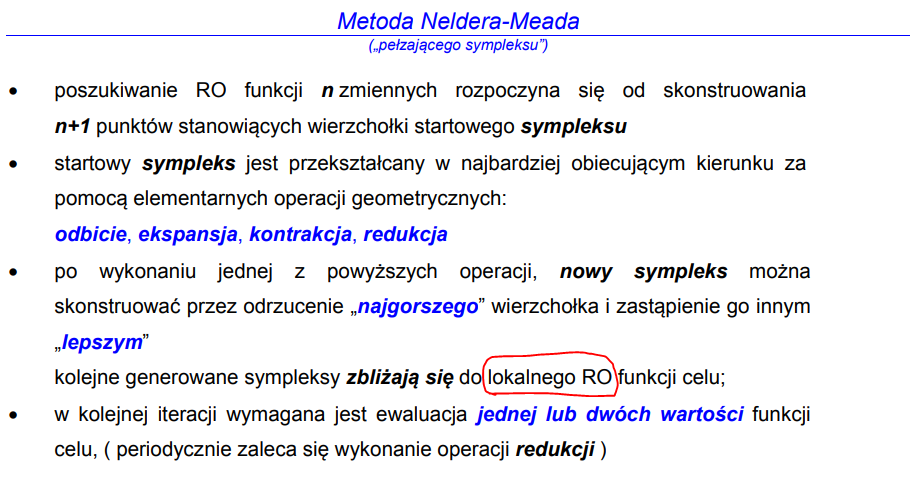
\includegraphics[scale=0.7]{Pictures/pelzajacy_sympleks}
	\caption{Pełzający sympleks}
\end{figure}
\begin{figure}[H]
	\centering
	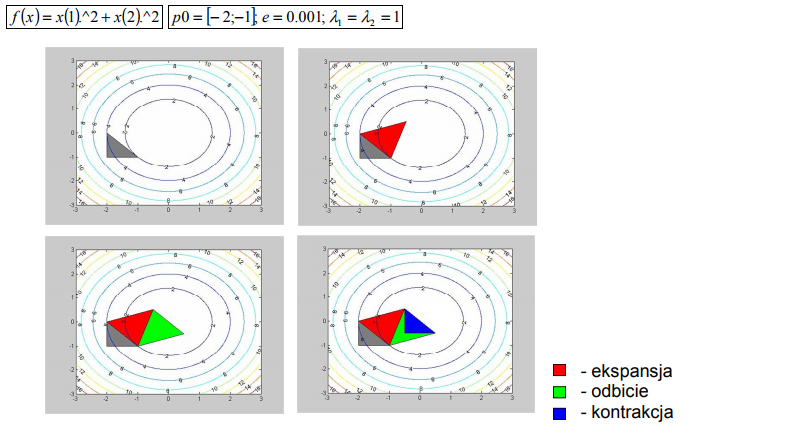
\includegraphics[scale=0.7]{Pictures/pelzajacy_sympleks2}
	\caption{Pełzający sympleks - przykład}
\end{figure}

\subsection{Optymalizacja nieliniowa z ograniczeniami}
Obszar poszukiwań minimum jest teraz ograniczony ograniczeniami nieloniowymi. Kierunek dopuszczalny musi być wewnątrz lub na ściance zbioru ograniczającego.
\begin{figure}[H]
	\centering
	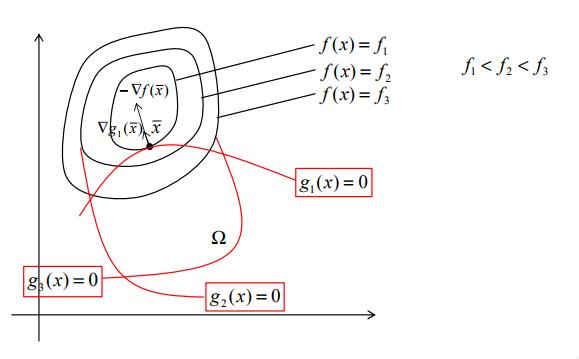
\includegraphics[scale=0.7]{Pictures/ograniczenia_nieliniowe}
	\caption{Optymalizacja z ograniczeniami}
\end{figure}

\textbf{Warunki Kuhna-Tuckera}\\
Jeżeli ZPN jest regularne to WKT są konieczne, żeby punkt był ekstremum (był rozwiązaniem). Jeżeli zadanie jest wypukłe (funkcja celu jest wypukła, zadanie nie posiada nieliniowych ograniczeń równościowych, a ograniczenia nierównościowe są wypukłe) to WKT jest warunkiem koniecznym i wystarczającym. 

\textbf{Funkcja Lagarange'a} $$L(x,\lambda) = f(x) + \lambda^{T}(Ax-b)$$ Jest wykorzystywana do sprawdzenia czy dany punkt jest RO zadania otymalizacji nieliniowej z ograniczeniami. Sprawdzamy to za pomocą WKT.\\
~\\
Algorytmy programowania kwadratowego:
\begin{enumerate}
	\item metoda eliminacji uogólnionej,
	\item metoda zbioru ograniczeń aktywnych,
	\item metoda rzutowania gradientu.
\end{enumerate}

\subsection{Metody funkcji kary}
Gdy mamy zadanie optymalizacji nieliniowej z ograniczeniami, to możemy je przekształci na zadanie optymalizacji bez ograniczeń stosując funkcję kary.
$$min F_{k}(x,r_{k})$$ gdzie $$F_{k}(x,r_{k}) = f(x) + P_{k}(x,r_{k})$$ Mamy różne metody wyznaczania funkcji kary: wewnętrzną, zewnętrzną, odmiany. Funkcja kary karze za używanie rozwiązań niedopuszczalnych. Podstawowym problemem związanym z funkcją kary jest kwestia jak bardzo karać – zbyt niska kara może doprowadzić do dominacji rozwiązań niedopuszczalnych, zbyt wysoka jej wartość odrzuci większość (jeśli nie wszystkie) rozwiązań niedopuszczalnych a wśród nich także te które mogły być bardzo cenne.

\section{Metody numeryczne}

\subsection{Poszukiwanie zer funkcji jednej zmiennej}

\textbf{Metoda bisekcji}\\
Założenia: funkcja jest ciągła na przedziale $[a,b]$ i ma różne znaki na końcach przedziału.\\
Przedział $[a,b]$ dzielimy na połowę w punkcie $x_{0}$. Jeżeli $x_{0}$ nie jest pierwiastkiem to wybieramy jeden z przedziałów $[a,x_{0}]$ lub $[x_{0},b]$. Wybieramy ten, na którym funkcja ma różne znaki na końcach. Zbieżność 1.\\
\begin{figure}[H]
	\centering
	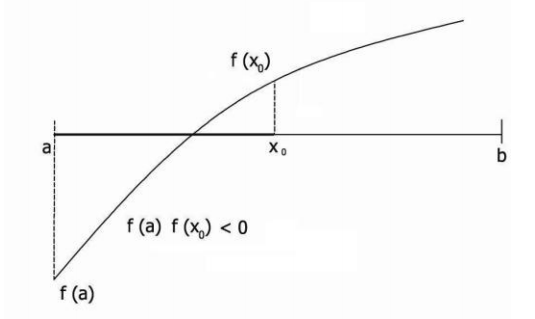
\includegraphics[scale=0.7]{Pictures/metoda_bisekcji}
	\caption{Metoda bisekcji}
\end{figure}

\textbf{Metoda stycznych Newtona}\\
Zbieżność kwadratowa.
\begin{figure}[H]
	\centering
	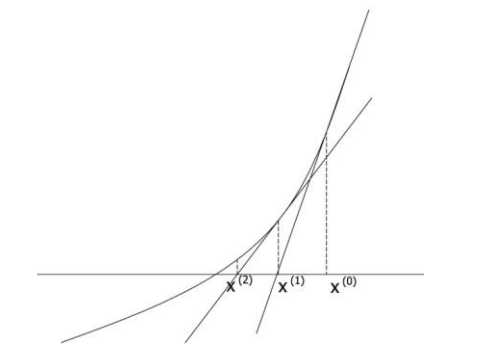
\includegraphics[scale=0.7]{Pictures/metoda_stycznych_newtona}
	\caption{Metoda Newtona}
\end{figure}

\textbf{Metoda stycznych siecznych}\\
Zbieżność 1.61.
\begin{figure}[H]
	\centering
	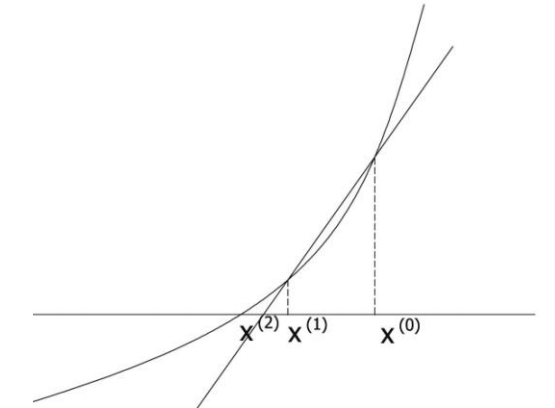
\includegraphics[scale=0.7]{Pictures/metoda_siecznych}
	\caption{Metoda siecznych}
\end{figure}
~\\
Często w \textbf{profesjonalnych solverach} używa się najpierw metody bisekcji, a potem metodę Newtona.

\subsection{Metody całkowania}
Całkujemy za pomocą różnych metod Newtona-Cotesa: metody prostokątów, metody trapezów, metody Simpsona (praboli). Metoda Simpsona interpoluje funkcję parabolą na trzech punktach za pomocą wielomianu Lagrange'a. Istnieje też metoda Monte-Carlo -- funkcję zamykamy w kwadrat i strzelamy. Obliczamy stosunek liczny trafionych do liczby strzałów i na tej podstawie szacujemy wartość.

\subsection{Metody rozwiązywania układów równań liniowych skończonych}
\textbf{Wzory Cramera}\\
$$x_{i} = \frac{W_{i}}{W}$$ gdzie:\\
$W$ -- wyznacznik główny\\
$W_{i}$ - wyznaczniki, w których współczynniki przy $x_{i}$ zastępujemy wyrazami wolnymi.

\textbf{Metoda eliminacji Gaussa}\\
Metoda eliminacji Gaussa dzieli się na dwa etapy:
\begin{enumerate}
	\item Sprowadzenie macierzy do postaci trójkątnej.
	\item Rozwiązanie takiego układu.
\end{enumerate}
Aby sprowadzić macierz do postaci trójkątnej możemy wykorzystać jedną z dwóch metod wyboru elementu głównego:
\begin{enumerate}
	\item Wybór częściowy: w k-tym kroku największy element z k-tej kolumny z wierszy $k-n$ i zamieniamy wiersze (ewntualnie działamy na wierszach i zamieniamy kolumny).
	\item Wybór pełny: maksymalnego elementu szukamy w podmacierzy i zamieniamy odpowiedni wiersz i kolumnę.
\end{enumerate}

\textbf{Rozkład LU}
$$PA = LU$$
Rozkład LU możemy uzyskać za pomocą eliminacji Gaussa, ale bez "doklejania" do $A$ wektora $b$. Wtedy z eliminacji otrzymujemy macierz schodkową, czylu $U$, a $L$ to złożenie operacji elementarnych na $A$, które doprowadziłY do $U$.\\
Inną metodą rozkładu LU jest metoda Doolittle'a.
~\\
\textbf{Rozkład Cholesky'ego-Banachawiecza}\\
Jeżeli A jest macierzą symetryczną i dodatnio określoną to istnieje macierz trójkątna dolna L z dodatnimi elementami na głównej przekątnej:
$$A = LL^{T}$$
Jeżeli rozkład nie istnieje, to $A$ nie może być macierzą symetryczną dodatnio określoną.\\
Zastosowania rozkładu LU: obliczanie wyznacznika, rozwiązywanie układu równań $Ax = b$, obliczanie $A^{-1}$.

\subsection{Metody rozwiązywania układów równań liniowych iteracyjne}
Niech $x_{0}$ będzie wektorem nazywanym przybliżeniem początkowym. We wszystkich metodach iteracyjnych tworzony jest ciąg kolejnych przybliżen, który dąży do rozwiązania $x$.\\
~\\
\textbf{Metoda Jacobiego}\\
Niech $a_{ii} \neq 0$ dla $i = 1,...,n$. Przedstawiamy macierz A jako $A = U + L + D$. Liczymy $x_{k}$. Jeżeli A jest silnie diagonalnie dominująca to metoda jest zbieżna.
~\\
\textbf{Metoda Gaussa-Seidela}\\
Tak jak Jacobi, tylko mamy inny wzór na $x_{k}$. Metoda jest zbieżna w dwóch przypadkach:
\begin{enumerate}
	\item jeżeli A jest silnie diagonalnie dominująca
	\item $A = A^{T}$ i $A$ jest dodatnio określona.
\end{enumerate}
~\\
\textbf{Metoda SOR}\\
Metoda SOR jest uogólnieniem metody Gaussa-Seidela, w której wprowadzamy dodatkowy parametr relaksacji $\omega$, z pomocą którego mieszamy wartość poprzedniego kroku z wartością nową ($(1-\omega)x_{i} + \omega x_{i+1}$).
~\\
\textbf{Metoda gradientu sprzężonego}

\subsection{Metody rozwiązywania układów równań nieliniowych iteracyjne}
Rozwiązywanie układów równań sprowadza się do znalezienia takiego rozwiązania $\alpha \in R^{n}$, w którym odwzorowanie $F: R^{n} \rightarrow R^{n}$ przyjmuje wartość zero, tzn. $F(\alpha) = 0$.\\
~\\
\textbf{Metoda Newtona}\\
Dla układów równań nieliniowych metoda Newtona działa jako uogólnienie dobrze nam znanej metody stycznych Newtona. 

\end{document}